% Preamble templated from Dhawal24112006/EE1030
\documentclass{beamer}
\mode<presentation>
\usepackage{amsmath}
\usepackage{amssymb}
% \usepackage{advdate}
\usepackage{adjustbox}
\usepackage{subcaption}
% \usepackage{enumitem}
\usepackage{multicol}
\usepackage{mathtools}
\usepackage{listings}
\usepackage{url}
% \def\UrlBreaks{\do\/\do-}
\usetheme{Boadilla}
\usecolortheme{lily}
\setbeamertemplate{footline}
{
  \leavevmode%
  \hbox{%
  \begin{beamercolorbox}[wd=\paperwidth,ht=2.25ex,dp=1ex,right]{author in head/foot}%
    \insertframenumber{} / \inserttotalframenumber\hspace*{2ex}
  \end{beamercolorbox}}%
  \vskip0pt%
}
\setbeamertemplate{navigation symbols}{}

\providecommand{\nCr}[2]{\,^{#1}C_{#2}} % nCr
\providecommand{\nPr}[2]{\,^{#1}P_{#2}} % nPr
\providecommand{\mbf}{\mathbf}
\providecommand{\pr}[1]{\ensuremath{\Pr\left(#1\right)}}
\providecommand{\qfunc}[1]{\ensuremath{Q\left(#1\right)}}
\providecommand{\sbrak}[1]{\ensuremath{{}\left[#1\right]}}
\providecommand{\lsbrak}[1]{\ensuremath{{}\left[#1\right.}}
\providecommand{\rsbrak}[1]{\ensuremath{{}\left.#1\right]}}
\providecommand{\brak}[1]{\ensuremath{\left(#1\right)}}
\providecommand{\lbrak}[1]{\ensuremath{\left(#1\right.}}
\providecommand{\rbrak}[1]{\ensuremath{\left.#1\right)}}
\providecommand{\cbrak}[1]{\ensuremath{\left\{#1\right\}}}
\providecommand{\lcbrak}[1]{\ensuremath{\left\{#1\right.}}
\providecommand{\rcbrak}[1]{\ensuremath{\left.#1\right\}}}
\theoremstyle{remark}
\newtheorem{rem}{Remark}
\newcommand{\sgn}{\mathop{\mathrm{sgn}}}
\providecommand{\abs}[1]{\left\vert#1\right\vert}
\providecommand{\res}[1]{\Res\displaylimits_{#1}}
\providecommand{\norm}[1]{\lVert#1\rVert}
\providecommand{\mtx}[1]{\mathbf{#1}}
\providecommand{\mean}[1]{E\left[ #1 \right]}
\providecommand{\fourier}{\overset{\mathcal{F}}{ \rightleftharpoons}}
%\providecommand{\hilbert}{\overset{\mathcal{H}}{ \rightleftharpoons}}
\providecommand{\system}{\overset{\mathcal{H}}{ \longleftrightarrow}}
%\newcommand{\solution}[2]{\textbf{Solution:}{#1}}
%\newcommand{\solution}{\noindent \textbf{Solution: }}
\providecommand{\dec}[2]{\ensuremath{\overset{#1}{\underset{#2}{\gtrless}}}}
\newcommand{\myvec}[1]{\ensuremath{\begin{pmatrix}#1\end{pmatrix}}}
\let\vec\mathbf

\lstset{
% %language=C,
frame=single,
breaklines=true,
columns=fullflexible,
showstringspaces=false
}

\numberwithin{equation}{section}

\title{POMPS Presentation: 1.1.55}
\author{Subhodeep Chakraborty \\ ee25btech11055,\\IIT Hyderabad.}

\date{\today}
\begin{document}

\begin{frame}
\titlepage
\end{frame}

\section*{Outline}
\begin{frame}
\tableofcontents
\end{frame}

\section{Problem}
\begin{frame}
\frametitle{Problem Statement}
Let the signal $x(t)$ have the Fourier transform $X(\omega)$.
Consider the signal $y(t) = x(t-t_a)$ where $t_a$ is an arbitrary delay.
The magnitude of the Fourier transform of $y(t)$ is:
\vspace{0.5cm}
\begin{enumerate}[(a)]
    \item $\abs{X(\omega) \cdot [\omega]}$
    \item $\abs{X(\omega)} \cdot \omega$
    \item $\omega^2 \cdot \abs{X(\omega)}$
    \item $\abs{X(\omega) \cdot e^{-j\omega t_a}}$
\end{enumerate}
\end{frame}

\section{Solution}
\begin{frame}{Theoretical Solution}
Let $x(t)$ be mapped to the frequency domain via the \textbf{Continuous Fourier Transform Operator} $\mathcal{F}$, such that $x(t) \fourier X(\omega)$.
\vspace{0.5cm}

According to the \textbf{Time-Shifting Theorem}, a delay in the time domain corresponds to a phase rotation in the frequency domain, leaving the magnitude unchanged.
\vspace{0.5cm}

Mathematically:
\begin{align}
    x(t - t_a) &\fourier X(\omega)e^{-j\omega t_a}
    \label{eq:phase}
\end{align}
\end{frame}

\begin{frame}{Proof: Time-Shifting Theorem}
By the definition of the Continuous-Time Fourier Transform:
\begin{align}
    \mathcal{F}\cbrak{x(t - t_a)} &= \int_{-\infty}^{\infty} x(t - t_a) e^{-j\omega t} dt
\end{align}

Let $\tau = t - t_a$. \\
\begin{align}
    \mathcal{F}\cbrak{x(t - t_a)} &= \int_{-\infty}^{\infty} x(\tau) e^{-j\omega (\tau + t_a)} d\tau
\end{align}
\end{frame}

\begin{frame}{Proof: Time-Shifting Theorem}
\begin{align}
    \mathcal{F}\cbrak{x(t - t_a)} &= \int_{-\infty}^{\infty} x(\tau) e^{-j\omega \tau} e^{-j\omega t_a} d\tau
\end{align}

\begin{align}
    \mathcal{F}\cbrak{x(t - t_a)} &= e^{-j\omega t_a} \int_{-\infty}^{\infty} x(\tau) e^{-j\omega \tau} d\tau
\end{align}

\begin{align}
    \mathcal{F}\cbrak{x(t - t_a)} &= e^{-j\omega t_a} X(\omega)
\end{align}
\end{frame}

\begin{frame}{Eigenfunctions in LTI Systems}
To map this to linear algebra, we recall that an eigenvector $\mathbf{v}$ does not change direction under a linear transformation $T$; it is only scaled by an eigenvalue $\lambda$, such that $T(\mathbf{v}) = \lambda \mathbf{v}$.
\vspace{0.5cm}

Similarly, if passing a signal $x(t)$ through a Linear Time-Invariant (LTI) system $H$ simply scales the signal by a complex constant $\lambda$:
\begin{align}
    \mathcal{H}\cbrak{x(t)} &= \lambda \cdot x(t)
\end{align}
Then $x(t)$ is considered an \textbf{eigenfunction} of that system.
\end{frame}

\begin{frame}{Proof: Complex Exponentials as Eigenfunctions}
The output $y(t)$ of an LTI system is the convolution of the input signal $x(t)$ with the system's impulse response $h(t)$:
\begin{align}
    y(t) &= h(t) * x(t) = \int_{-\infty}^{\infty} h(\tau) x(t - \tau) d\tau
\end{align}

Let our input signal be a general complex exponential $x(t) = e^{st}$. Substituting this into the integral:
\begin{align}
    y(t) &= \int_{-\infty}^{\infty} h(\tau) e^{s(t - \tau)} d\tau \\
    y(t) &= \int_{-\infty}^{\infty} h(\tau) e^{st} e^{-s\tau} d\tau
\end{align}
\end{frame}

\begin{frame}{Proof: Complex Exponentials (Cont.)}
Because we are integrating with respect to $\tau$, the term $e^{st}$ is treated as a constant and factored out:
\begin{align}
    y(t) &= e^{st} \int_{-\infty}^{\infty} h(\tau) e^{-s\tau} d\tau
\end{align}

The remaining integral evaluates to a complex number dependent only on $s$. This is the definition of the system's \textbf{Transfer Function}, $H(s)$:
\begin{align}
    H(s) &= \int_{-\infty}^{\infty} h(\tau) e^{-s\tau} d\tau
\end{align}
Therefore, replacing the integral gives:
\begin{align}
    y(t) &= H(s) \cdot e^{st} = H(s) \cdot x(t)
\end{align}
\end{frame}

\begin{frame}{Linear Algebraic Formulation}
Since complex exponentials are eigenfunctions of LTI systems, we can formalise the time-delay operation using linear algebra. Let the representation of the continuous frequency spectrum at discrete frequencies $\omega_k$ be a column vector $\mathbf{X}$.
\vspace{0.5cm}

The time-shift operation acts as a \textbf{Linear Transformation} mapping input spectrum $\mathbf{X}$ to output spectrum $\mathbf{Y}$. This transformation is represented by a diagonal Matrix $\mathbf{C}$:

\begin{align}
    \mathbf{Y} &= \mathbf{C} \mathbf{X}
\end{align}
\end{frame}

\begin{frame}{Matrix Expansion}
Thus, from \eqref{eq:phase} we can write:
\begin{align}
    \begin{pmatrix} Y(\omega_1) \\ Y(\omega_2) \\ \vdots \\ Y(\omega_k) \end{pmatrix} 
    &=
    \begin{pmatrix}
    e^{-j\omega_1 t_a} & 0 & \dots & 0 \\
    0 & e^{-j\omega_2 t_a} & \dots & 0 \\
    \vdots & \vdots & \ddots & \vdots \\
    0 & 0 & \dots & e^{-j\omega_k t_a}
    \end{pmatrix}
    \begin{pmatrix} X(\omega_1) \\ 
X(\omega_2) \\ \vdots \\ X(\omega_k) \end{pmatrix}
\end{align}
\end{frame}

\begin{frame}{Magnitude Evaluation}
For any arbitrary frequency component $\omega$, the operation simplifies to:
\begin{align}
  \label{eq:ans}
    \abs{Y(\omega)} &= \abs{X(\omega) \cdot e^{-j\omega t_a}} \\
    \abs{Y(\omega)} &= \abs{X(\omega)} \cdot \abs{e^{-j\omega t_a}} \label{eq:magnitude_split}
\end{align}

\begin{align}
    \abs{e^{-j\omega t_a}} &= \sqrt{\cos^2(-\omega t_a) + \sin^2(-\omega t_a)} = 1
\end{align}
\end{frame}

\begin{frame}{Final Conclusion}
Substituting this unity magnitude back into the split equation gives:
\begin{align}
    \abs{Y(\omega)} &= \abs{X(\omega)} \cdot 1 \\
    \abs{Y(\omega)} &= \abs{X(\omega)}
\end{align}

Looking at the given options, option (d) represents \eqref{eq:ans} before simplification:
\begin{align}
    \abs{X(\omega) \cdot e^{-j\omega t_a}} &= \abs{X(\omega)} \cdot \abs{e^{-j\omega t_a}} = \abs{X(\omega)}
\end{align}

Therefore, the magnitude of the signal's frequency spectrum is entirely invariant to linear time delays, while phase shift is given by \eqref{eq:phase}. The correct choice is \textbf{(d)}. This is illustrated in a plot using a Gaussian pulse as well as a sinc pulse as the input.
\end{frame}
\iffalse
\begin{frame}{Sidenote: Energy Conservation}
The mathematical conclusion that $\abs{Y(\omega)} = \abs{X(\omega)}$ has a direct physical interpretation via \textbf{Parseval's Theorem}.
\vspace{0.5cm}

Parseval's Theorem states that the total energy of a signal in the time domain is equal to the total energy in the frequency domain:
\begin{align}
    E &= \int_{-\infty}^{\infty} \abs{x(t)}^2 dt = \frac{1}{2\pi} \int_{-\infty}^{\infty} \abs{X(\omega)}^2 d\omega
\end{align}

Since our delayed signal $y(t)$ has the exact same magnitude spectrum $\abs{X(\omega)}$, its total energy remains identical. 
\vspace{0.3cm}

\textit{Intuition:} Shifting a pulse in time does not change its shape or amplitude; therefore, the total energy carried by the signal is perfectly conserved. The phase shift purely dictates \textbf{when} that energy arrives.
\end{frame}
\fi
\section{Python Codes}
\begin{frame}[fragile,allowframebreaks]{Python Implementation}
\begin{lstlisting}[basicstyle=\scriptsize\ttfamily][language=Python]
import numpy as np
import matplotlib.pyplot as plt
from scipy.fft import fft, fftfreq, fftshift, ifftshift
import os

output_dir = '../figs/'

dt = 0.01
t = np.arange(-50, 50, dt)

# sinc pulse
x = np.sinc(t)
t_a = 2.0 
y = np.sinc(t - t_a) # y(t) = x(t - t_a)

n = len(t)
X = fftshift(fft(ifftshift(x)))
Y = fftshift(fft(ifftshift(y)))

freqs = fftshift(fftfreq(n, d=dt))

mag_X = np.abs(X)
mag_Y = np.abs(Y)

phase_X = np.angle(X)
phase_Y = np.angle(Y)

valid_idx = mag_X > 0.05*np.max(mag_X)

f_valid = freqs[valid_idx]
#ignore weak freqs instead of sharp jump to 0
phase_X_valid = np.unwrap(np.angle(X[valid_idx]))
phase_Y_valid = np.unwrap(np.angle(Y[valid_idx]))

center_idx = np.argmin(np.abs(f_valid)) # Set 0Hz to 0
phase_X_valid -= phase_X_valid[center_idx]
phase_Y_valid -= phase_Y_valid[center_idx]

plt.figure(figsize=(8, 5))
plt.plot(t, x, label='x(t) : Original Signal', color='blue')
plt.plot(t, y, label=f'y(t) : Delayed Signal (t_a={t_a})', color='red', linestyle='--')
plt.title('Time Domain')
plt.xlabel('Time (t)')
plt.ylabel('Amplitude')
plt.xlim(-5, 7)
plt.legend()
plt.grid(True)
plt.tight_layout()

time_domain_path = os.path.join(output_dir, 'time_domain_plot.png')
plt.savefig(time_domain_path, dpi=300)
print(f"Saved: {time_domain_path}")
plt.close()

plt.figure(figsize=(8, 5))
plt.plot(freqs, mag_X, label='|X(ω)| : Magnitude of x(t)', color='blue', linewidth=3)
plt.plot(freqs, mag_Y, label='|Y(ω)| : Magnitude of y(t)', color='orange', linestyle='--', linewidth=2)
plt.title('Frequency Domain: Magnitude')
plt.xlabel('Frequency (Hz)')
plt.ylabel('Magnitude')
plt.xlim(-2, 2)
plt.legend()
plt.grid(True)
plt.tight_layout()

magnitude_path = os.path.join(output_dir, 'magnitude_spectrum_plot.png')
plt.savefig(magnitude_path, dpi=300)
print(f"Saved: {magnitude_path}")
plt.close()

plt.figure(figsize=(8, 5))
plt.plot(f_valid, phase_X_valid, label=r'$\angle X(\omega)$ : Phase of x(t)', color='blue') # waaaow latex crajee
plt.plot(f_valid, phase_Y_valid, label=r'$\angle Y(\omega)$ : Phase of y(t)', color='red', linestyle='--')
plt.title('Frequency Domain: Phase')
plt.xlabel('Frequency (Hz)')
plt.ylabel('Phase (Radians)')
plt.xlim(-2, 2)
plt.legend()
plt.grid(True)
plt.tight_layout()

phase_path = os.path.join(output_dir, 'phase_spectrum_plot.png')
plt.savefig(phase_path, dpi=300)
print(f"Saved: {phase_path}")
plt.close()
\end{lstlisting}
\end{frame}

\section{Plots}
\subsection{Gaussian Pulse}
\begin{frame}{Time Domain Plot}
    \begin{figure}[h]
        \centering
        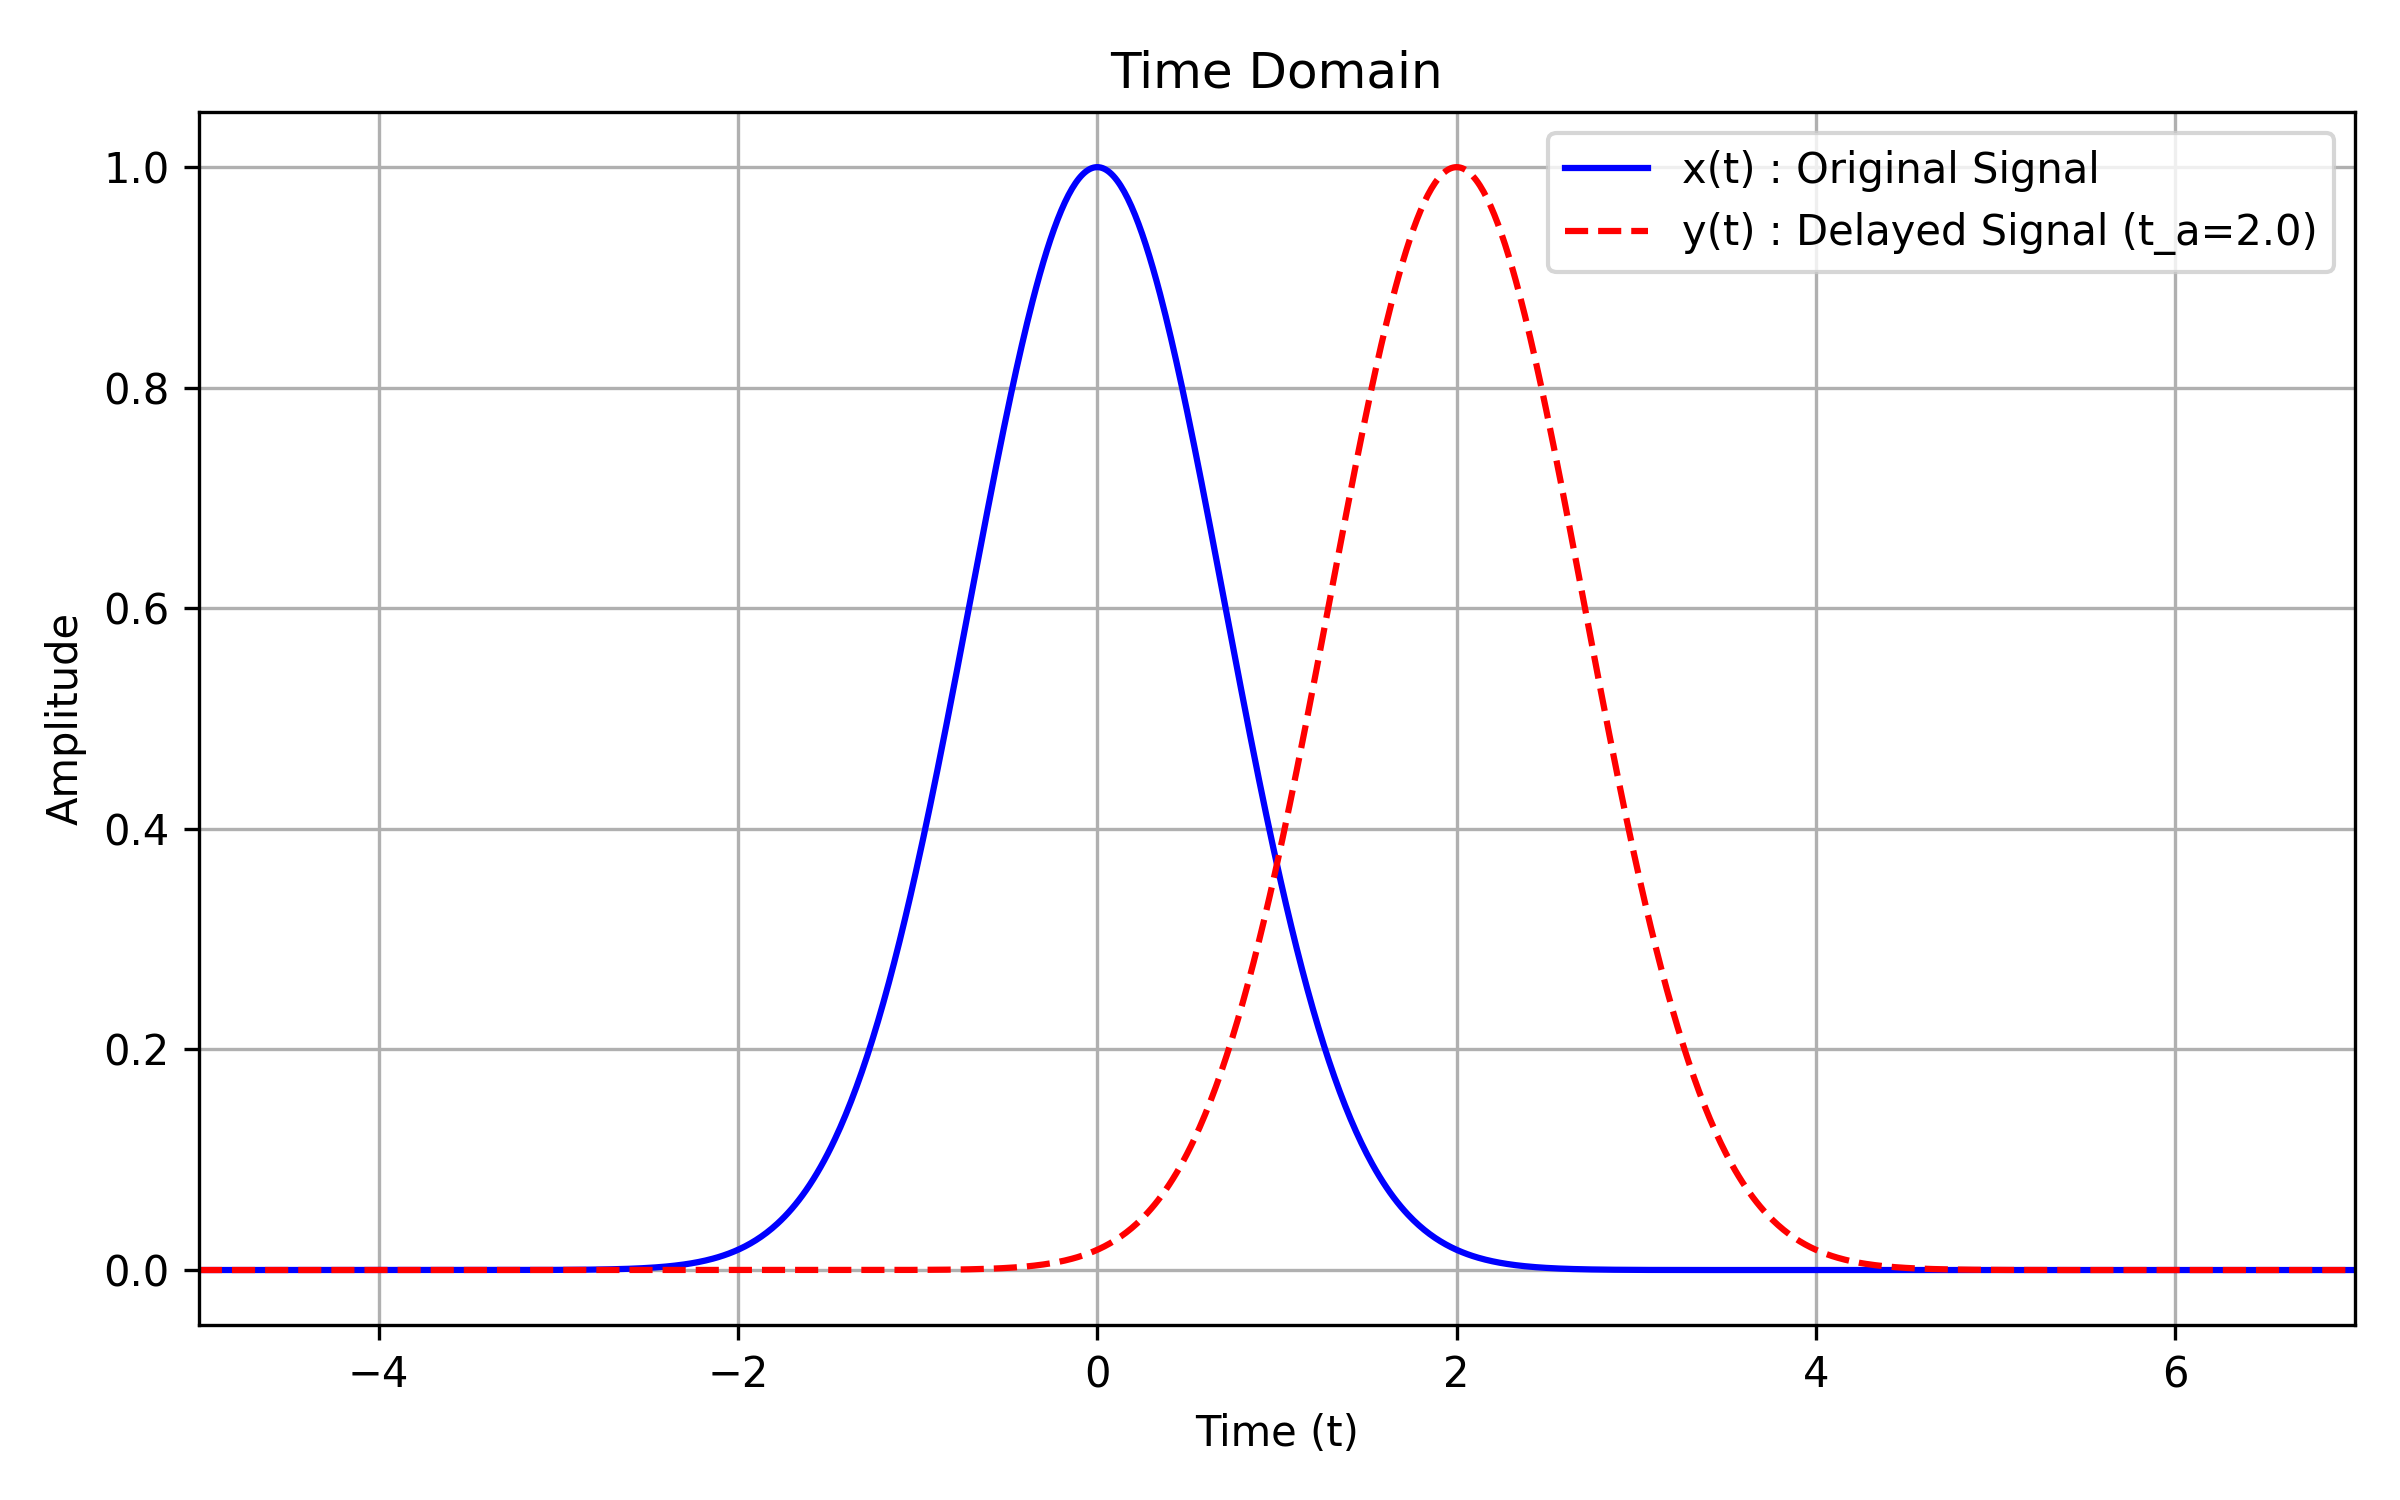
\includegraphics[width=0.85\linewidth]{../figs/time_domain_plot.png}
        \caption{Time Domain: Original vs Delayed Signal}
    \end{figure}
\end{frame}

\begin{frame}{Magnitude Spectrum Plot}
    \begin{figure}[h]
        \centering
        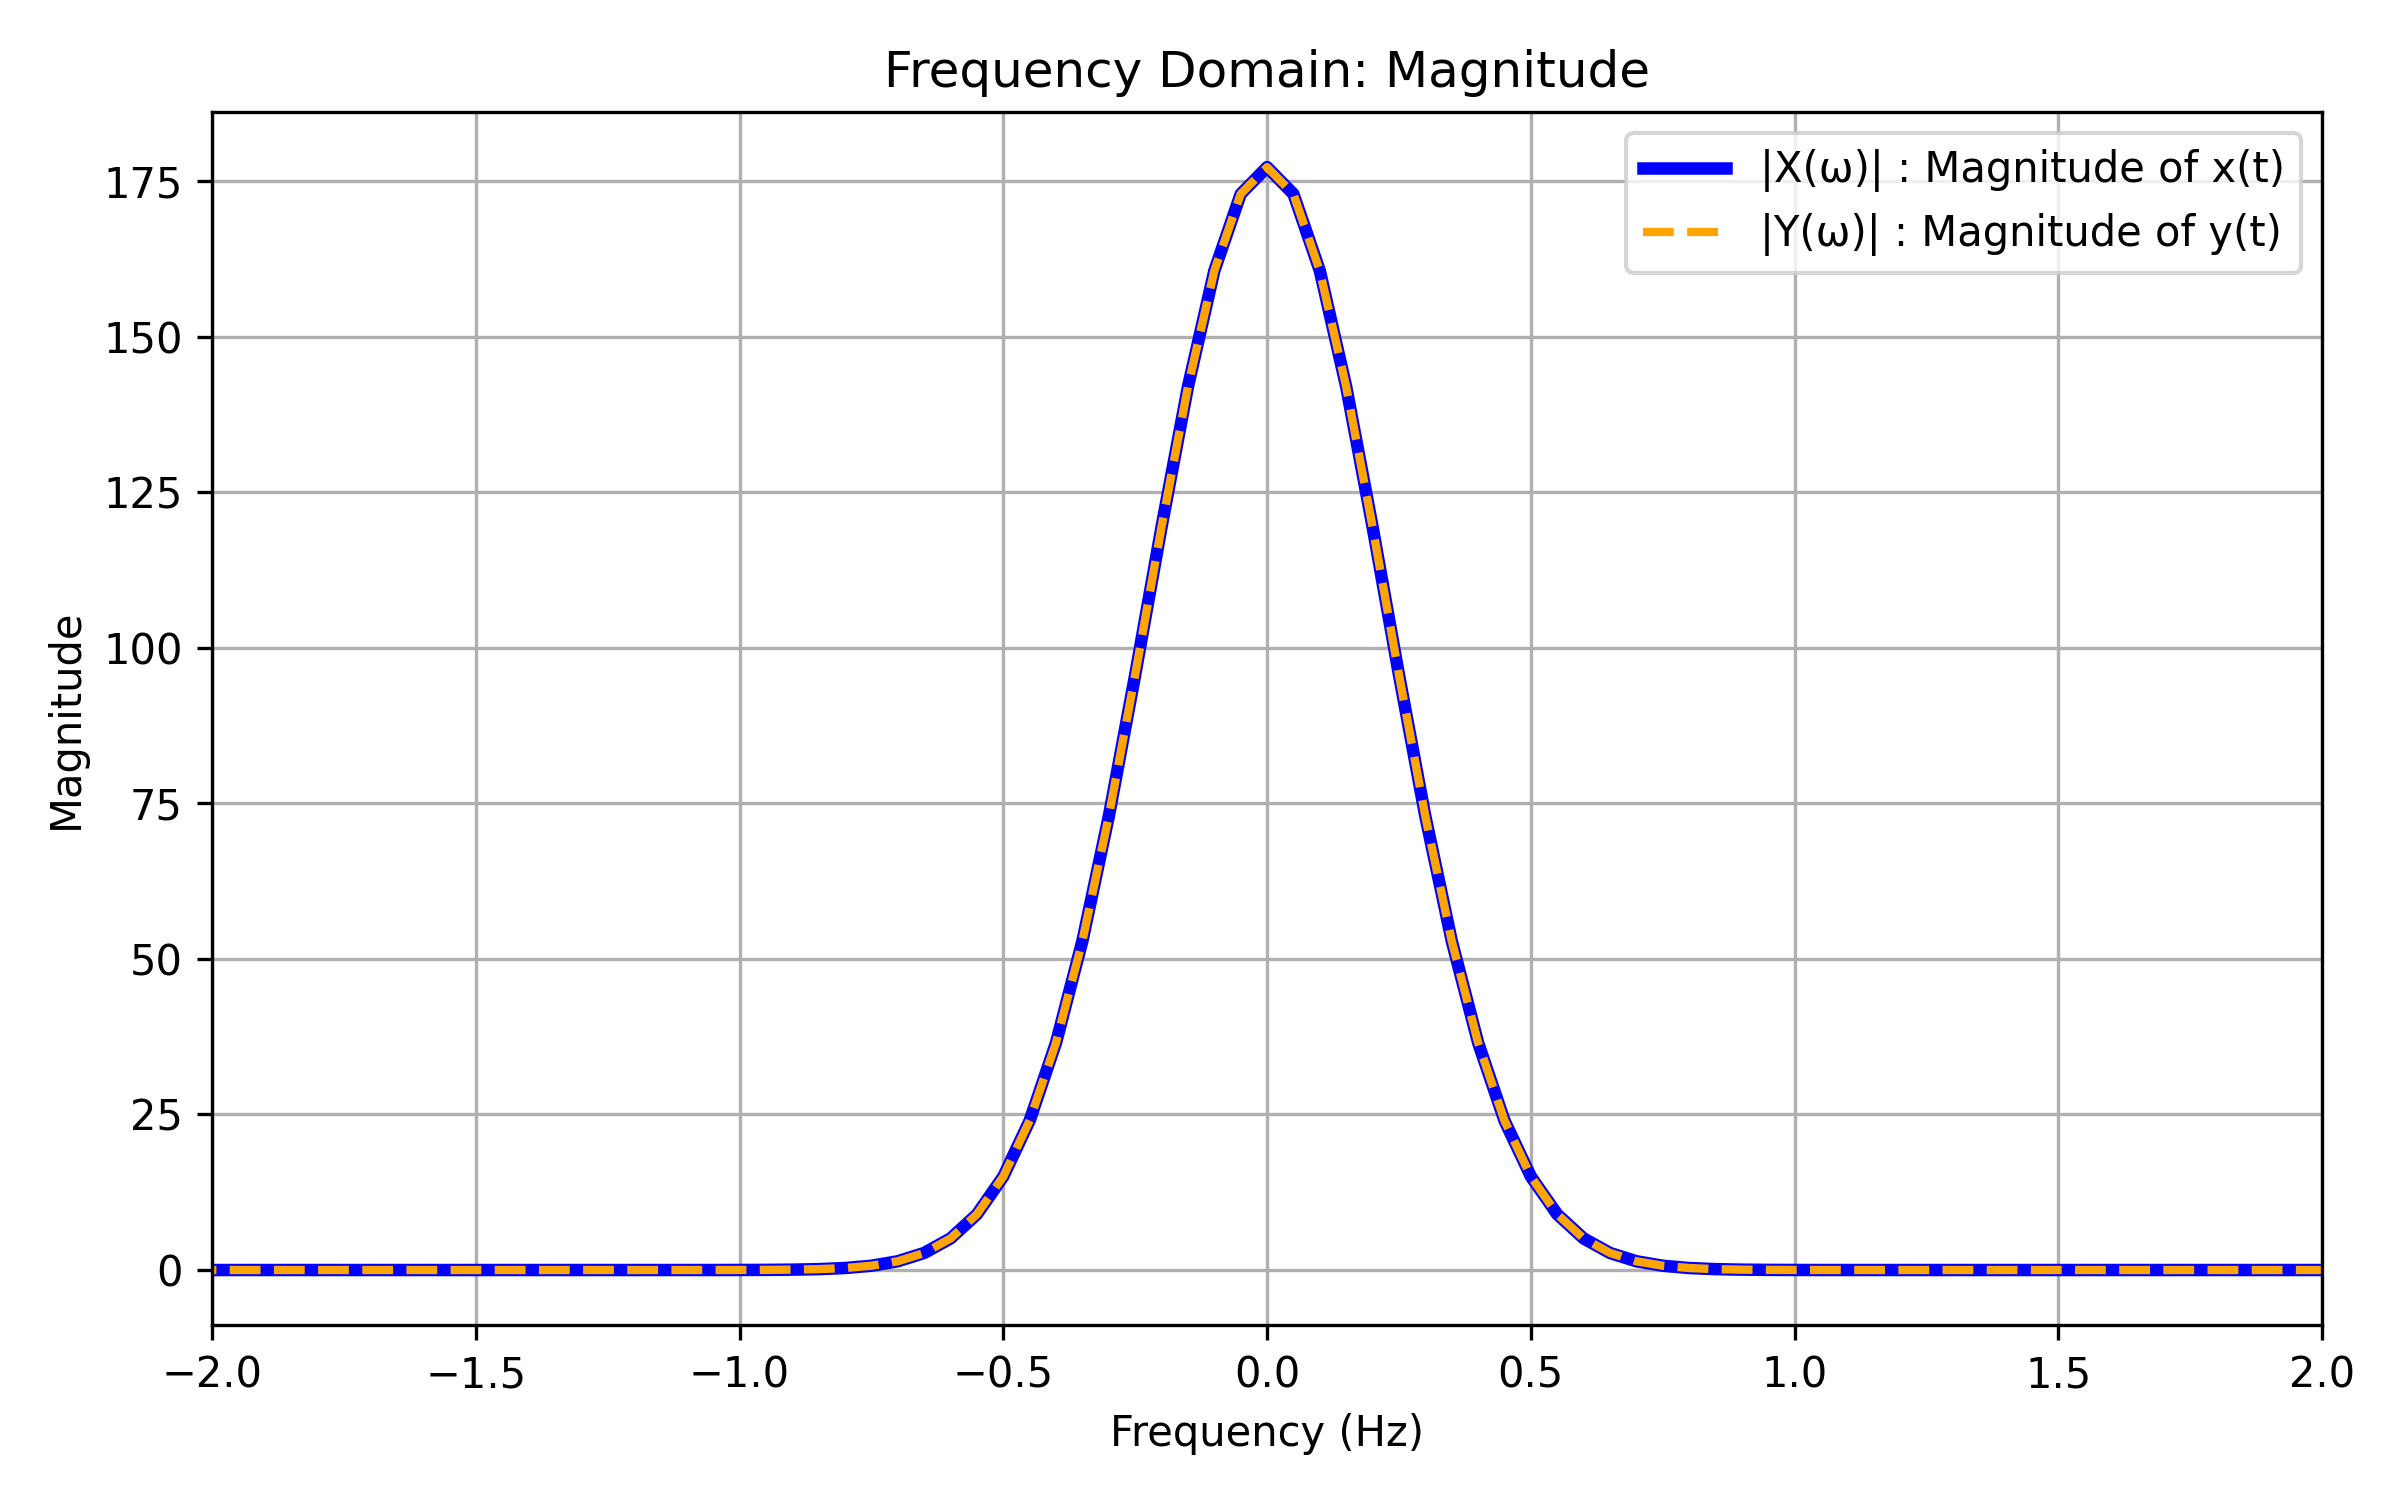
\includegraphics[width=0.85\linewidth]{../figs/magnitude_spectrum_plot.png}
        \caption{Frequency Domain: Magnitude Spectrum}
    \end{figure}
\end{frame}

\begin{frame}{Phase Spectrum Plot}
    \begin{figure}[h]
        \centering
        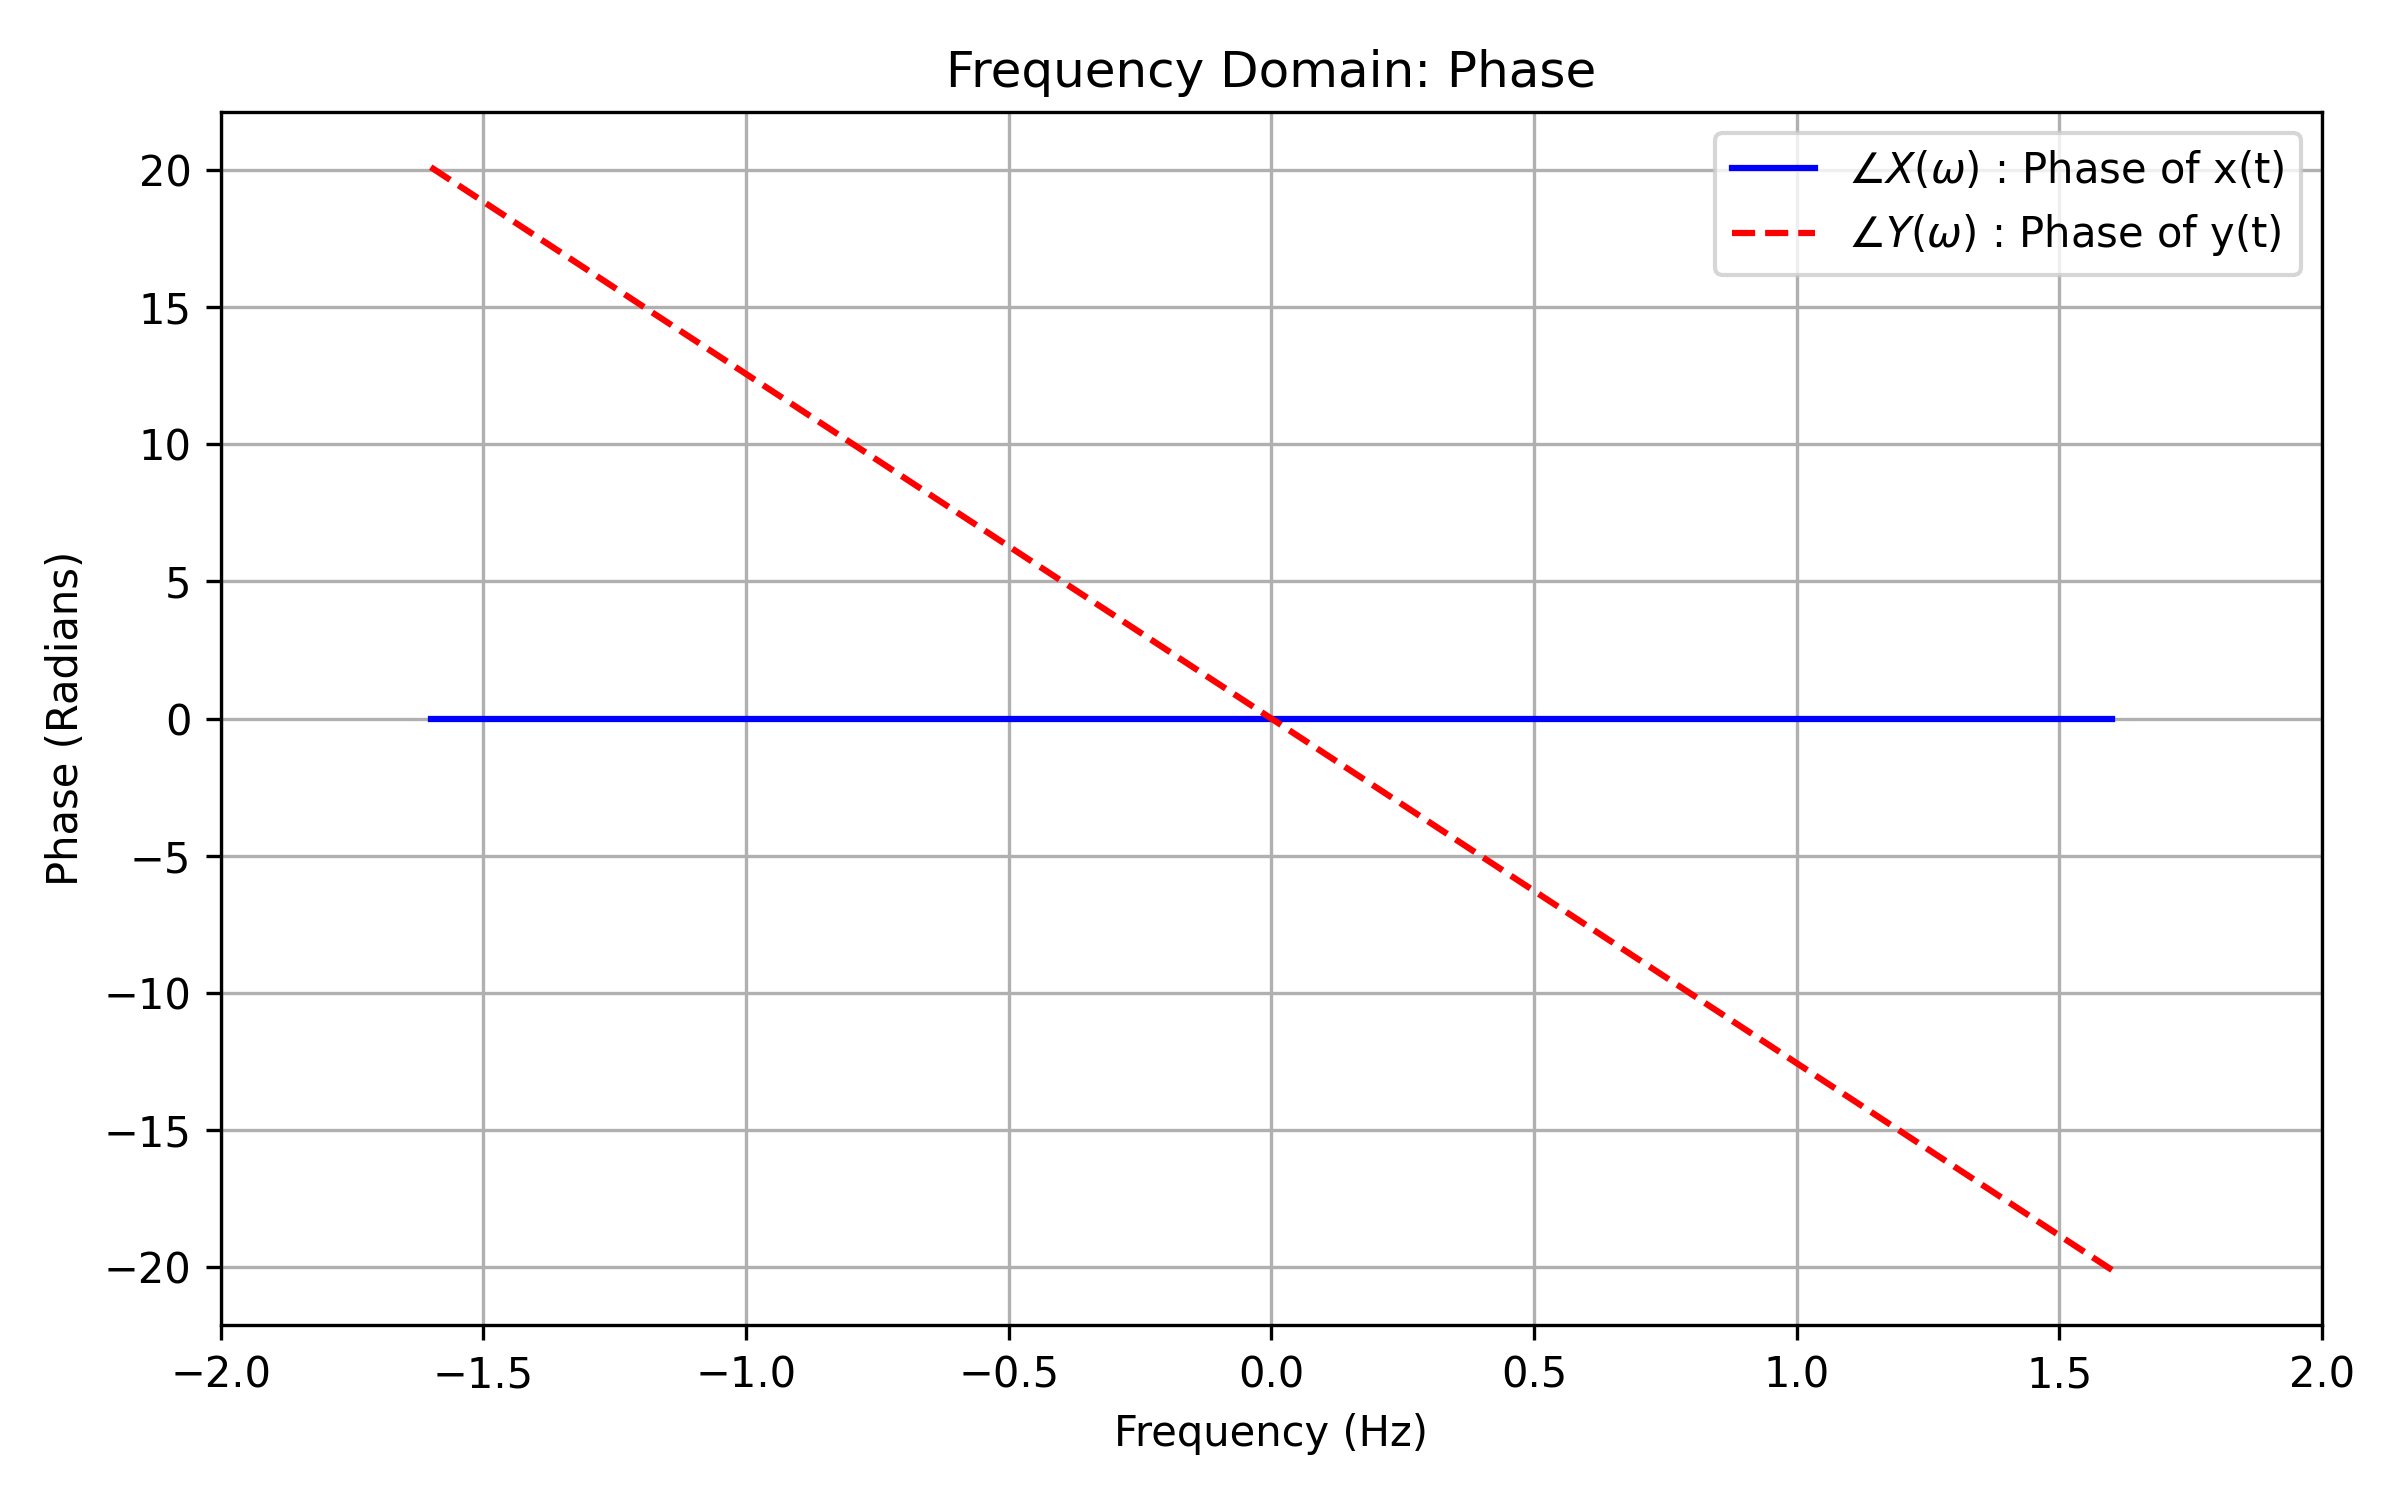
\includegraphics[width=0.85\linewidth]{../figs/phase_spectrum_plot.png}
        \caption{Frequency Domain: Phase Spectrum}
    \end{figure}
\end{frame}

\subsection{Sinc Pulse}
\begin{frame}{Time Domain Plot}
    \begin{figure}[h]
        \centering
        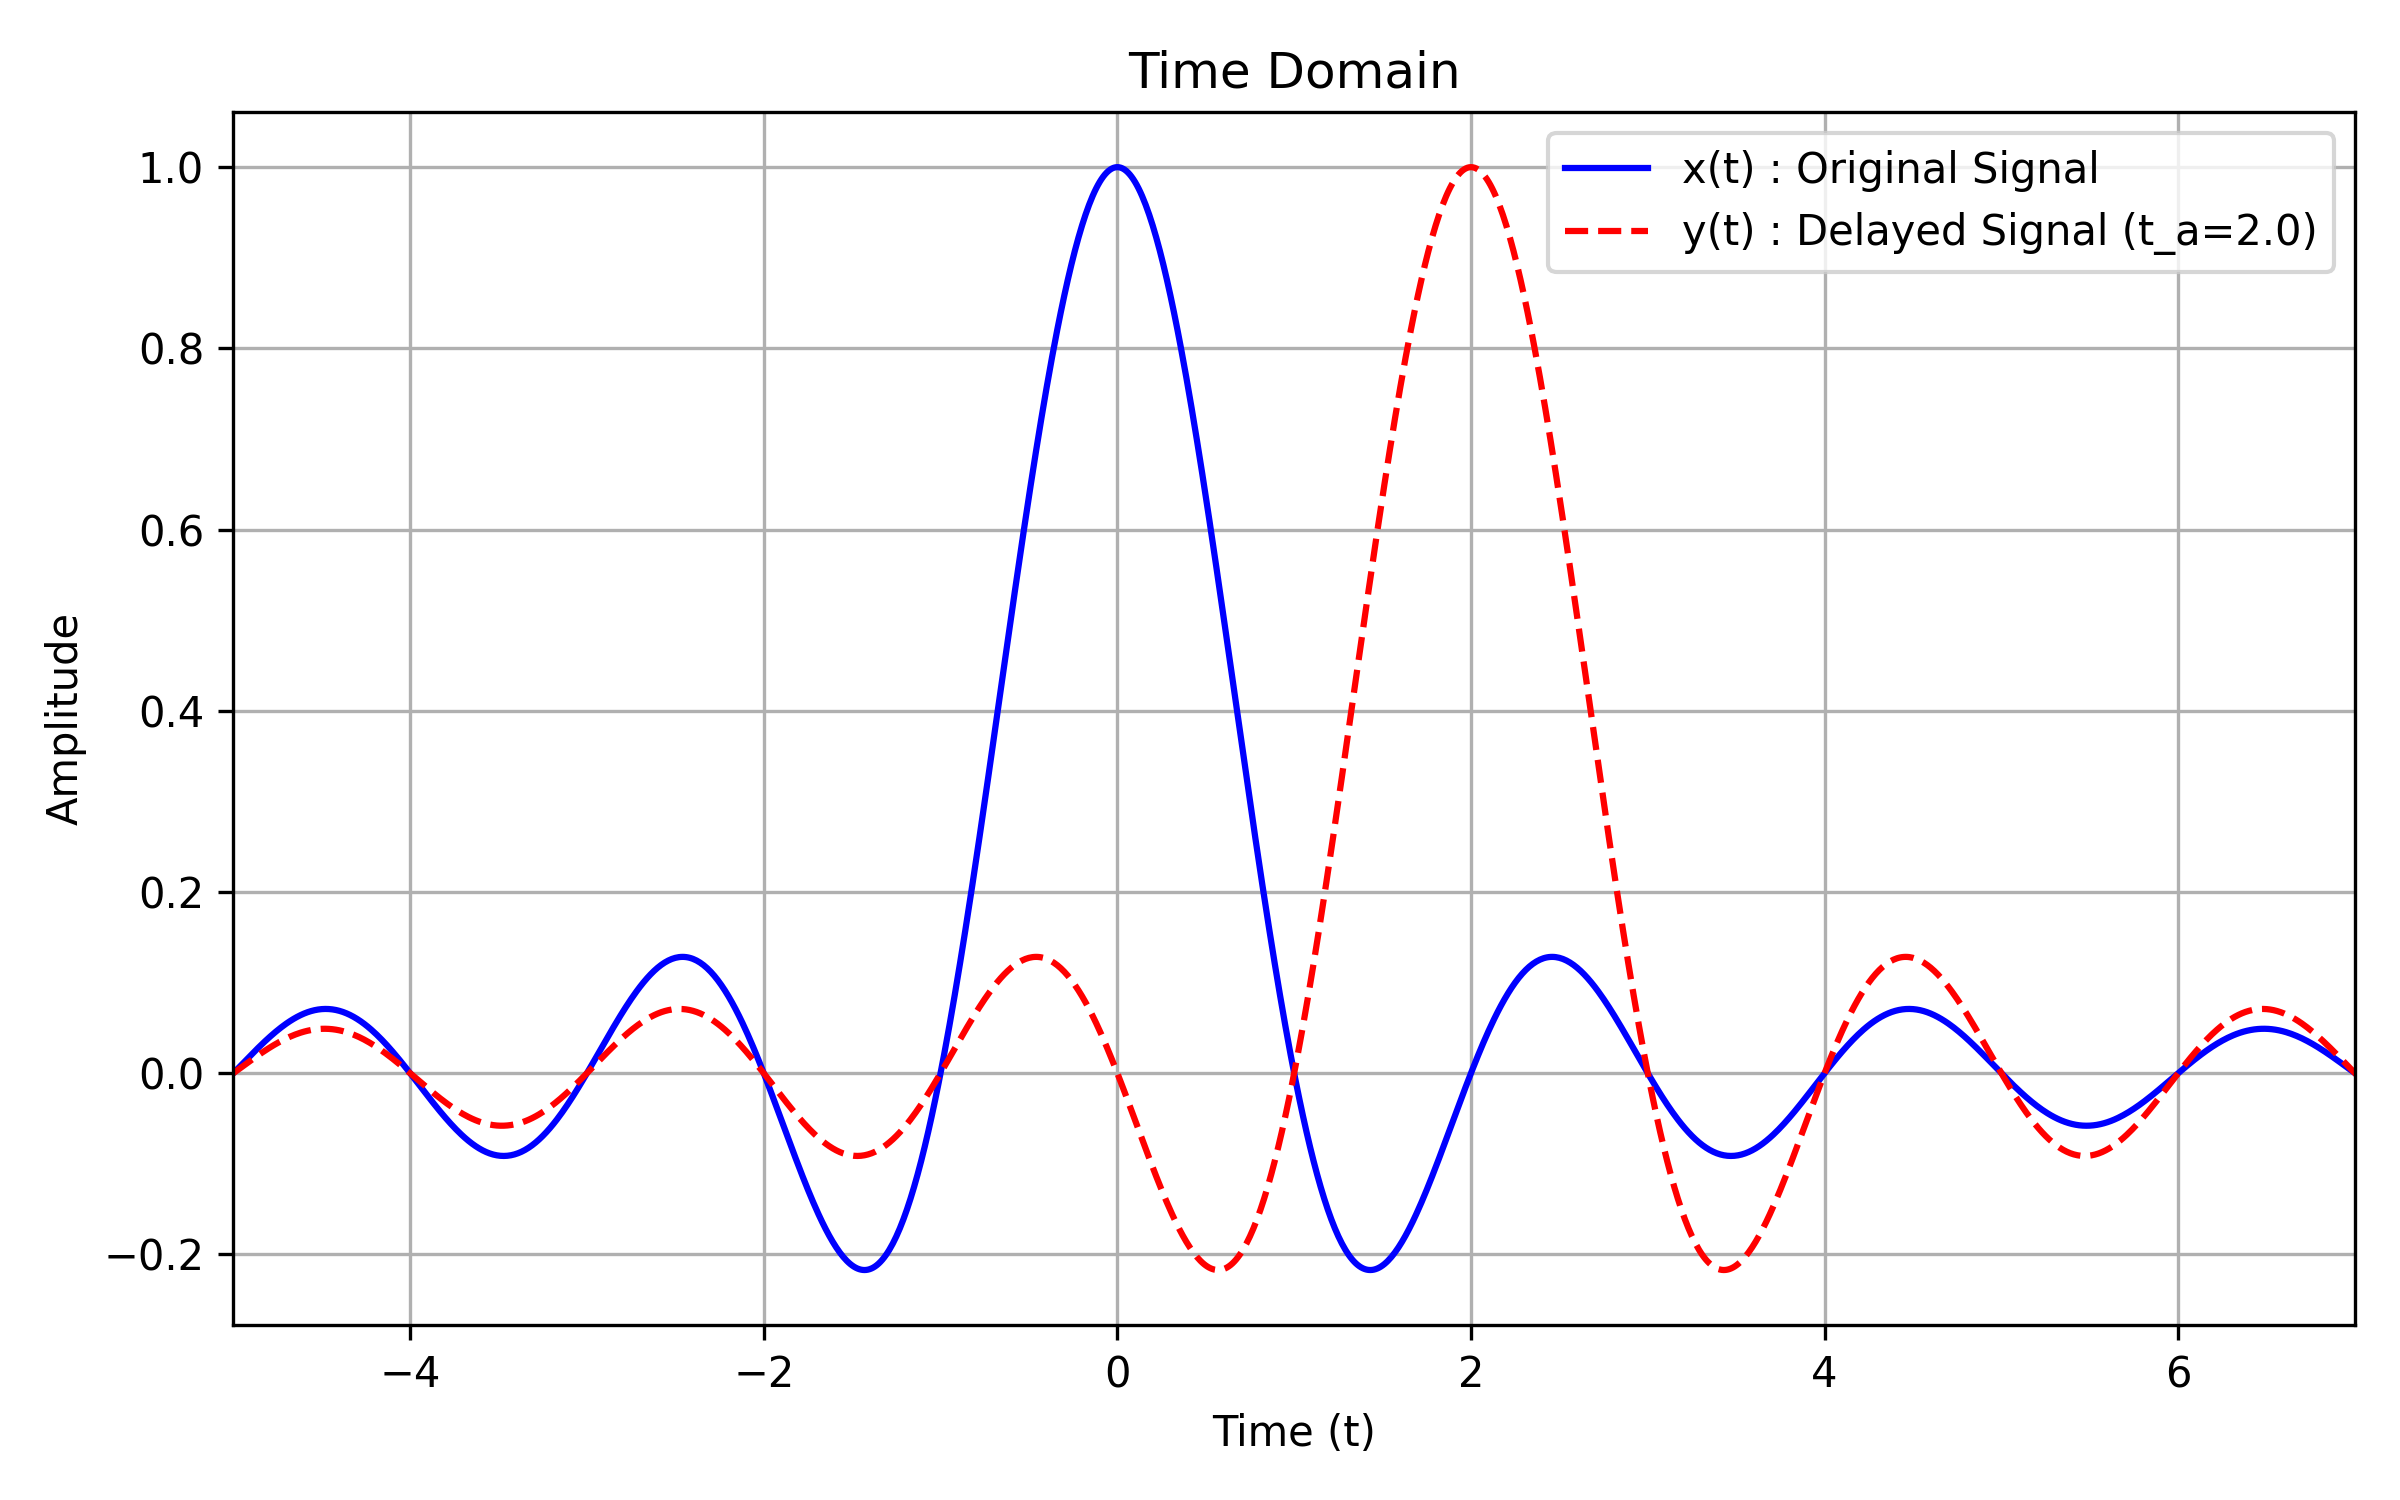
\includegraphics[width=0.85\linewidth]{../figs/time_domain_plot1.png}
        \caption{Time Domain: Original vs Delayed Signal}
    \end{figure}
\end{frame}

\begin{frame}{Magnitude Spectrum Plot}
    \begin{figure}[h]
        \centering
        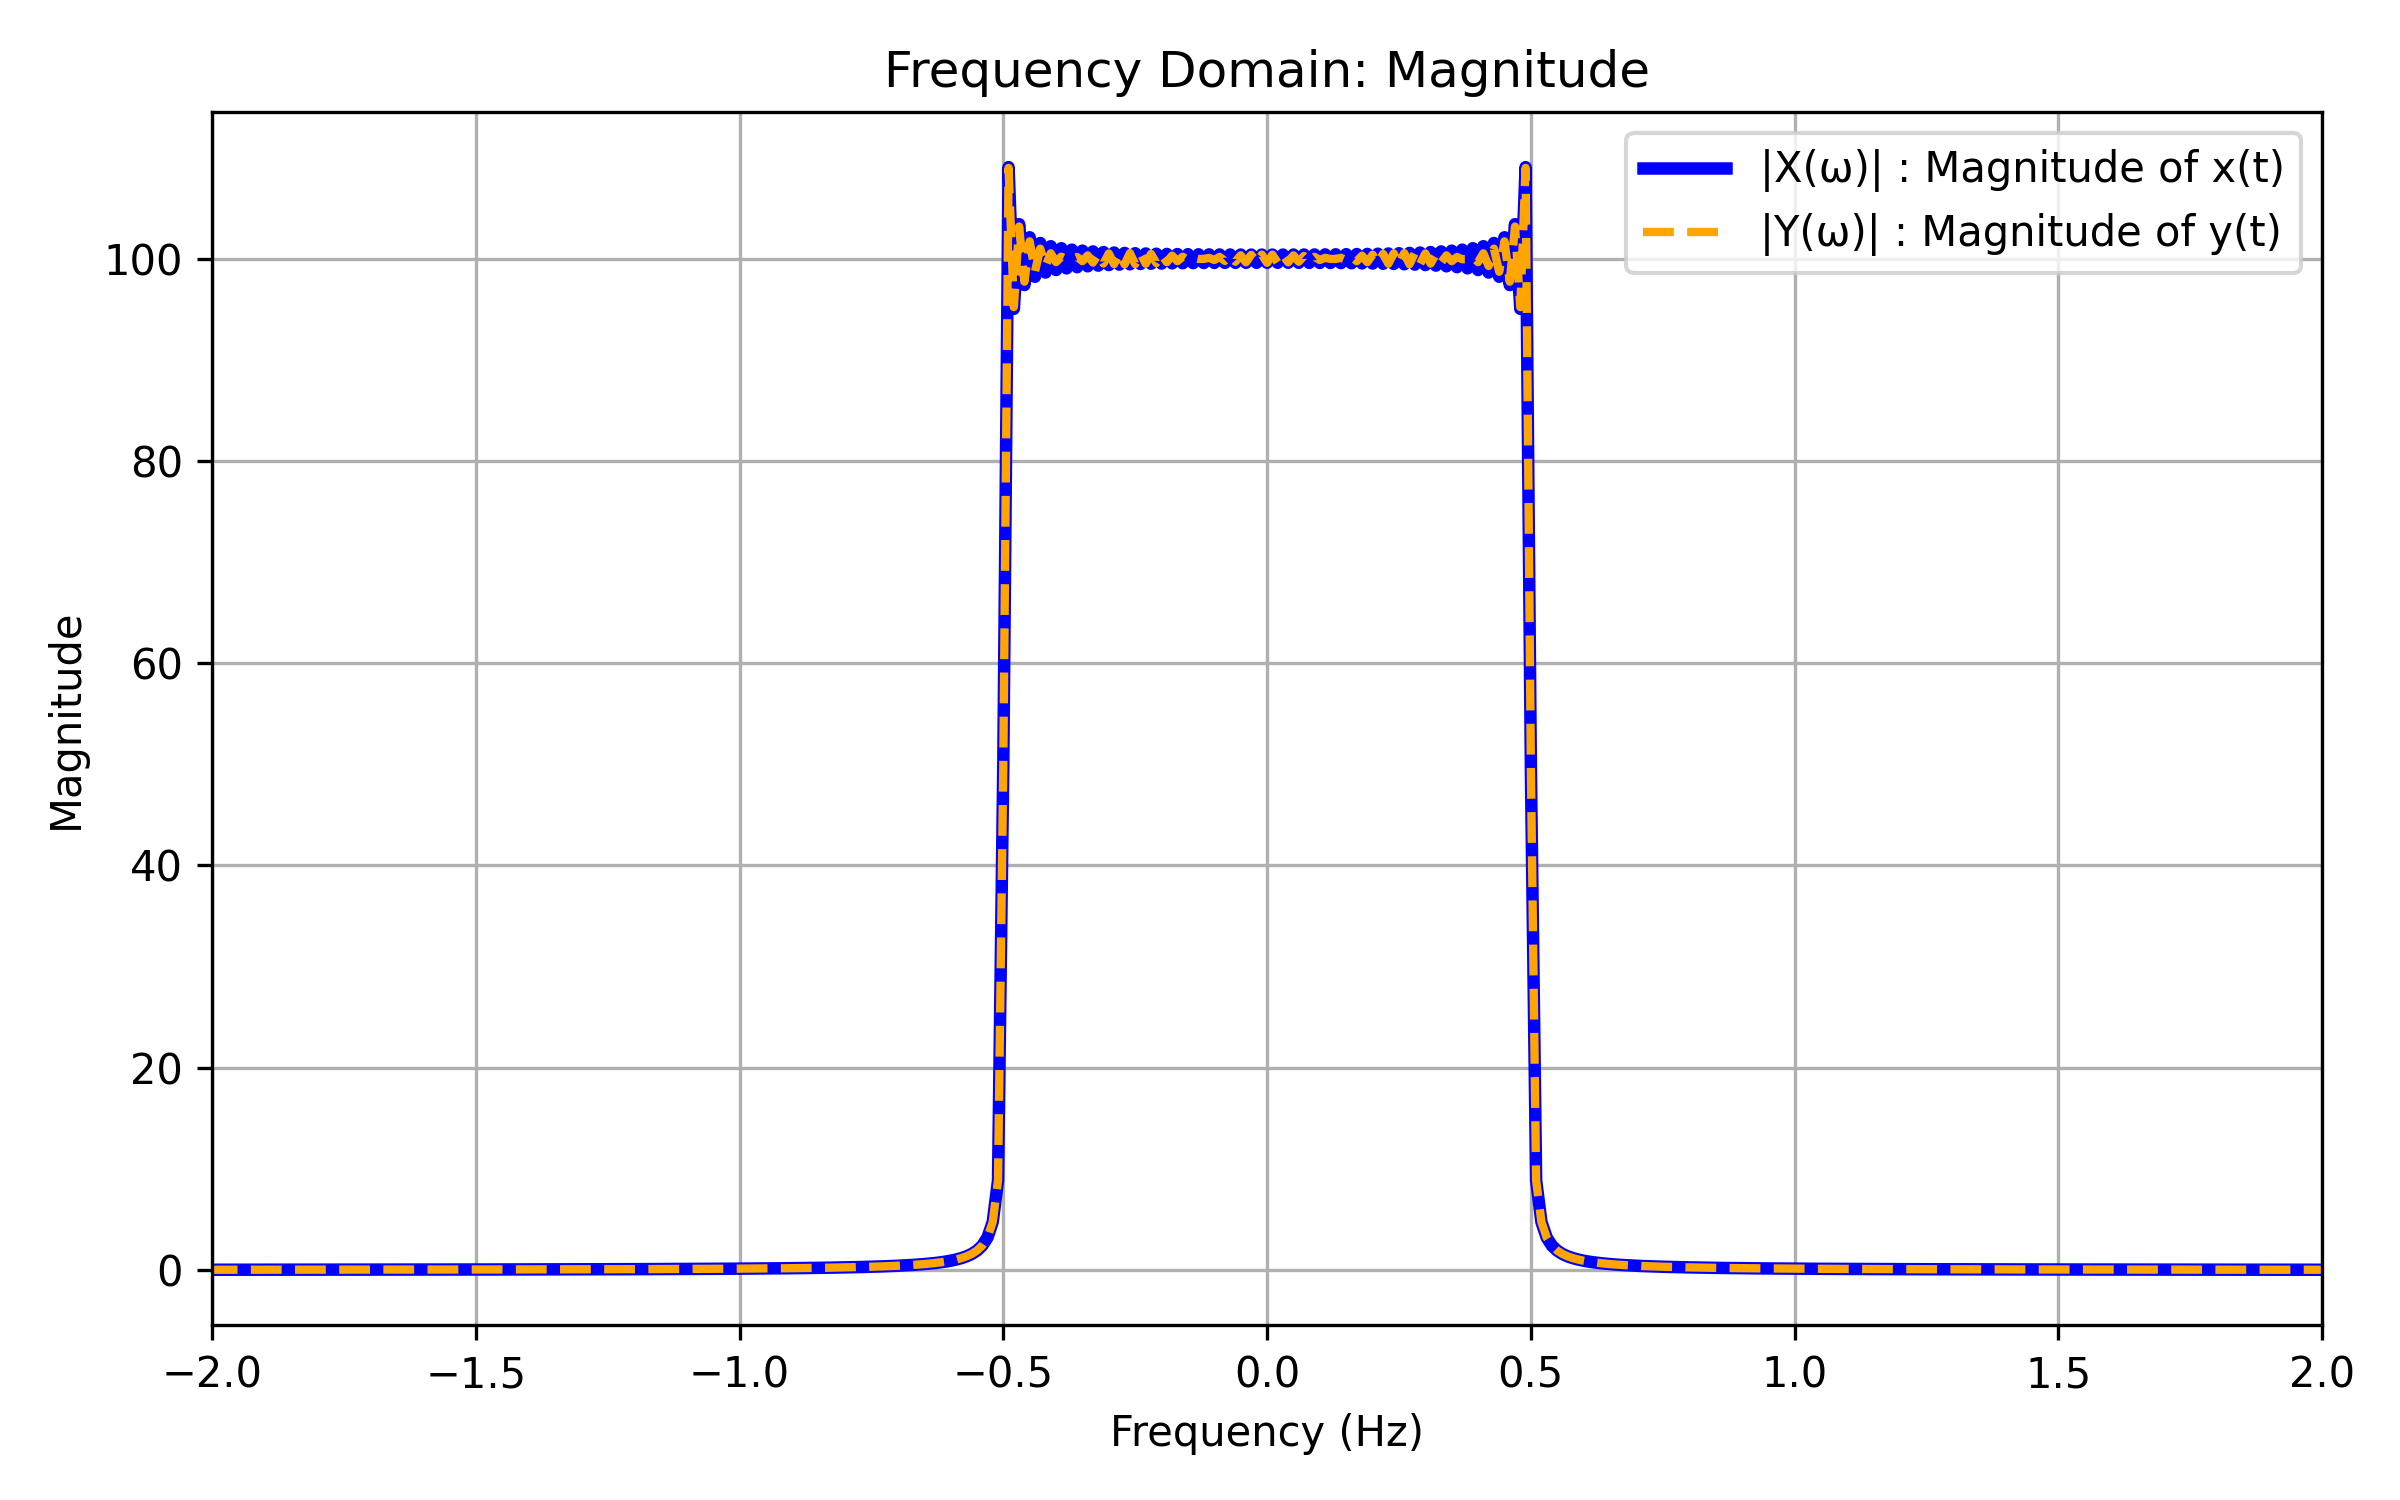
\includegraphics[width=0.85\linewidth]{../figs/magnitude_spectrum_plot1.png}
        \caption{Frequency Domain: Magnitude Spectrum}
    \end{figure}
\end{frame}

\begin{frame}{Phase Spectrum Plot}
    \begin{figure}[h]
        \centering
        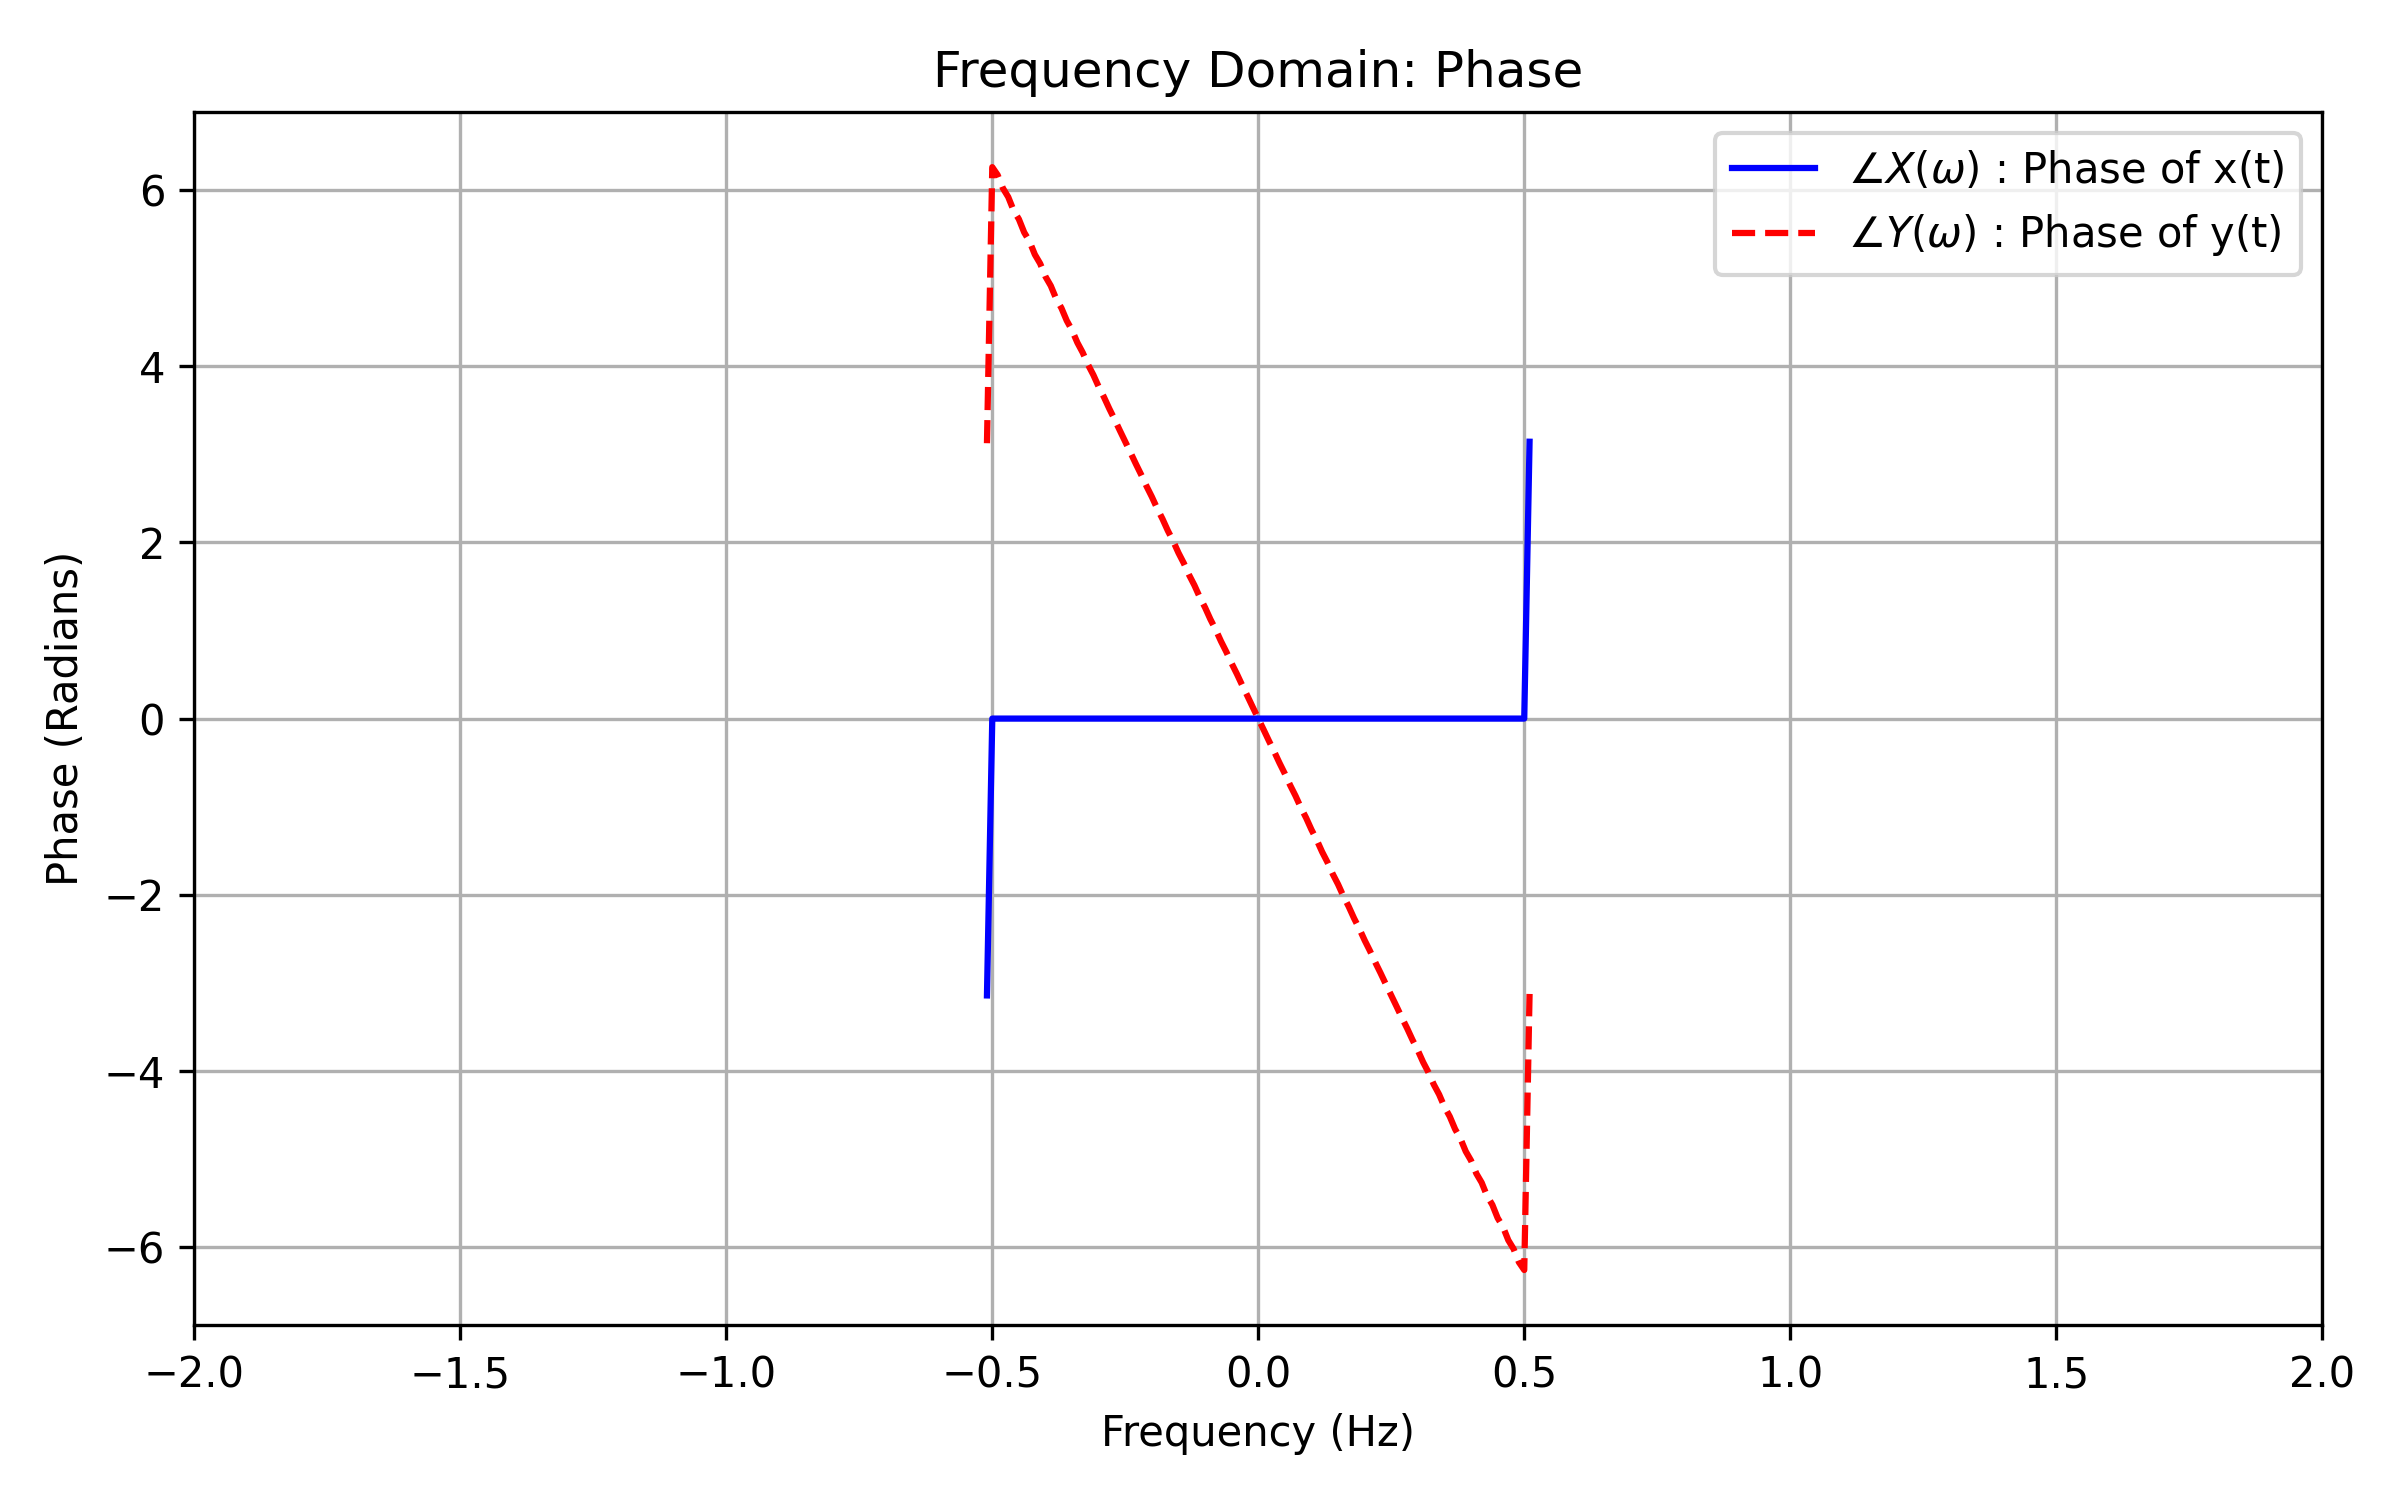
\includegraphics[width=0.85\linewidth]{../figs/phase_spectrum_plot1.png}
        \caption{Frequency Domain: Phase Spectrum}
    \end{figure}
\end{frame}
\end{document}
